\documentclass[12pt,letterpaper]{article}

% ── Packages ──────────────────────────────────────────────────────────────────
\usepackage[margin=1in]{geometry}
\usepackage{booktabs}
\usepackage{longtable}
\usepackage{array}
\usepackage{xcolor}
\usepackage{colortbl}
\usepackage{siunitx}
\usepackage{amsmath}
\usepackage{hyperref}
\usepackage{graphicx}
\usepackage{enumitem}
\usepackage{fancyhdr}
\usepackage{titlesec}
\usepackage{caption}
\usepackage{tikz}
\usepackage[american, siunitx]{circuitikz}
\usepackage{float}

\usepackage{parskip}

% ── Colors ────────────────────────────────────────────────────────────────────
\definecolor{violet}{RGB}{109,40,217}
\definecolor{ledblue}{RGB}{29,111,181}
\definecolor{ledgreen}{RGB}{21,128,61}
\definecolor{ledred}{RGB}{185,28,28}
\definecolor{rowgray}{RGB}{245,245,245}
\definecolor{headblue}{RGB}{30,64,175}
\definecolor{warnred}{RGB}{185,28,28}
\definecolor{notegreen}{RGB}{21,128,61}
\definecolor{lightviolet}{RGB}{237,233,254}
\definecolor{lightblue}{RGB}{219,234,254}
\definecolor{lightgreen}{RGB}{220,252,231}
\definecolor{lightred}{RGB}{254,226,226}

% ── Header / Footer ───────────────────────────────────────────────────────────
\pagestyle{fancy}
\fancyhf{}
\rhead{\small Color Analyzer LED Driver Design}
\lhead{\small \leftmark}
\rfoot{\small Page \thepage}
\lfoot{\small \today}

% ── Section formatting ────────────────────────────────────────────────────────
\titleformat{\section}{\large\bfseries\color{headblue}}{{\thesection}}{1em}{}[\titlerule]
\titleformat{\subsection}{\normalsize\bfseries}{{\thesubsection}}{1em}{}

% ── Hyperref setup ────────────────────────────────────────────────────────────
\hypersetup{colorlinks=true, linkcolor=headblue, urlcolor=headblue}

% ── siunitx setup ─────────────────────────────────────────────────────────────
\sisetup{per-mode=symbol}

% ── Column types ─────────────────────────────────────────────────────────────
\newcolumntype{C}[1]{>{\centering\arraybackslash}p{#1}}
\newcolumntype{L}[1]{>{\raggedright\arraybackslash}p{#1}}
\newcolumntype{R}[1]{>{\raggedleft\arraybackslash}p{#1}}

% ─────────────────────────────────────────────────────────────────────────────
\begin{document}

\begin{titlepage}
  \centering
  \vspace*{2cm}
  {\Huge\bfseries\color{headblue} Color Analyzer LED Driver\par}
  \vspace{0.5cm}
  {\Large Design Analysis and Component Selection\par}
  \vspace{2cm}
  {\large Raspberry Pi Camera Module 3 $\cdot$ Four-Channel Sequential Illumination\par}
  \vspace{0.5cm}
  {\large Violet $\cdot$ Blue $\cdot$ Green $\cdot$ Red\par}
  \vspace{3cm}
  {\normalsize\today\par}
  \vfill
  {\small This document covers design goals, component selection rationale, circuit calculations,\\
  resistor values for three brightness levels, schematic, and component recommendations.\\
  It is written for a technically-minded reader who may not have prior electronics design experience.}
\end{titlepage}

\tableofcontents
\newpage

% ═════════════════════════════════════════════════════════════════════════════
\section{Design Goals}
% ═════════════════════════════════════════════════════════════════════════════

This project is a color analyzer that uses a Raspberry Pi Camera Module~3 to photograph
color samples under four different colored lights in rapid sequence. By comparing how a
sample looks under violet, blue, green, and red illumination separately, software can
extract detailed color information beyond what a single white-light photograph provides.

The key design goals are:

\begin{enumerate}[leftmargin=2em]
  \item \textbf{Four distinct wavelength channels.} The LED colors must be narrow-band and
    well-separated so the camera sees meaningfully different information in each frame.
    Target wavelengths: violet/near-UV ($\sim$410~nm), blue ($\sim$475~nm),
    green ($\sim$525~nm), red ($\sim$625~nm).

  \item \textbf{Sequential, not simultaneous, illumination.} Only one color group fires at
    a time. This simplifies the power budget and the circuit, and avoids color mixing on
    the sample.

  \item \textbf{Controlled, repeatable brightness.} The camera exposure time can be adjusted
    per channel (up to 1.2~seconds), but consistent LED brightness is important for
    calibration. Three brightness levels (Low, Medium, High) are defined to give flexibility
    during commissioning.

  \item \textbf{Safe operation within power budget.} The power supply is a 2.5~A unit shared
    with a Raspberry Pi Zero~2~W, leaving approximately \textbf{0.5~A (500~mA) for the LEDs}.

  \item \textbf{GPIO compatibility.} The Raspberry Pi GPIO pins run at 3.3~V and can safely
    source about 16~mA per pin. The LEDs must be switched by a transistor driven from GPIO,
    not directly.

  \item \textbf{Low cost.} Four LEDs per color (six for violet) totaling 18 LEDs; individual
    LED cost should be under \$0.50 each.

  \item \textbf{Consistent package.} Where possible, use the same physical LED footprint
    across all four colors to simplify PCB layout.
\end{enumerate}

% ═════════════════════════════════════════════════════════════════════════════
\section{What Was Considered and Why}
% ═════════════════════════════════════════════════════════════════════════════

\subsection{Wavelength Selection}

The Raspberry Pi Camera Module~3 uses a Sony IMX708 sensor. Like all color camera sensors
it has a Bayer color filter array (red, green, and blue pixels) and a built-in infrared-cut
filter. Its useful sensitivity extends from about 400~nm at the violet end to roughly
700~nm at the red end, with a broad peak in the green region around 520--560~nm.

\textbf{Violet/near-UV (target 395--420~nm):} This is the most challenging channel.
No part in the available catalog covers the ideal 385--405~nm range. The best available
option, row~1015, has a dominant wavelength of 410~nm and a peak at 420~nm, which is
within camera sensitivity and provides useful channel separation. Its datasheet confirms:
absolute maximum current 30~mA, maximum power dissipation 120~mW, forward voltage
2.8~V (min) to 4.0~V (max). Because the worst-case $V_f$ is 4.0~V, the resistor
calculation must use this value to guarantee the LED is never over-driven.
At 4.0~V forward voltage on a 5~V supply, only 1.0~V is available across the resistor.
Six LEDs are used to compensate for the lower flux per device. True deep UV LEDs
($<$380~nm) would require a specialty supplier (e.g.\ Nichia) and are expensive.

\textbf{Blue (target 460--475~nm):} A well-populated part of the catalog. The 475~nm
region sits cleanly between the violet and green channels, and the IMX708 has good
blue-pixel sensitivity here.

\textbf{Green (target 520--530~nm):} The 525~nm range is the peak sensitivity region of
most camera sensors and of the human eye. LEDs here are bright, efficient, and cheap.

\textbf{Red (target 620--630~nm):} The 625~nm region is well inside the camera's red
sensitivity and comfortably below the infrared-cut filter cutoff at $\sim$700~nm.
Wavelengths above 660~nm would be increasingly attenuated by the IR filter.

\subsection{LED Classes}

Two fundamentally different LED classes appeared in the supplier catalog:

\begin{itemize}[leftmargin=2em]
  \item \textbf{Power LEDs} (first catalog): Tested at 100--350~mA, specified in lumens
    (lm). These are high-brightness devices in 3528/3030/2525 SMD packages. They produce
    far more light per LED but draw more current.

  \item \textbf{Indicator/signal LEDs} (second catalog): Tested at 5--20~mA, specified
    in millicandela (mcd). These are conventional signal LEDs in 0402/0603/0805/1206
    packages. They are cheaper and easier to drive but need more units for equivalent
    illumination.
\end{itemize}

Both classes can work. The power LED approach uses fewer LEDs at higher current;
the indicator approach uses more LEDs at lower current. For this design, first-choice
selections mix both classes depending on what was available at the right wavelength.

\subsection{LED Package Consistency}

The 1411 (3528 Metric) package was chosen as the target wherever possible. This is a
3.5~mm $\times$ 2.8~mm surface-mount package with a standardized footprint. Using the
same package for all four colors means one PCB pad layout serves all groups, and
component placement is predictable.

\subsection{Number of LEDs Per Group}

Four LEDs per color group provides adequate illuminance and keeps the circuit simple.
The violet channel uses six LEDs because the 410~nm LED (row~1015) is a small
indicator-class device. Its datasheet confirms an absolute maximum forward current of
30~mA and a maximum power dissipation of 120~mW. The forward voltage ranges from
2.8~V (minimum) to 4.0~V (maximum), with 2.8~V typical. Six LEDs at moderate current
compensates for the lower flux per device compared to the power LEDs used in the other
channels.

% ═════════════════════════════════════════════════════════════════════════════
\section{Circuit Architecture}
% ═════════════════════════════════════════════════════════════════════════════

\subsection{Overview}

The circuit uses four identical driver stages, one per color group. Each stage consists of:

\begin{itemize}[leftmargin=2em]
  \item $N$ LEDs in \textbf{parallel}, each with its own current-setting resistor
  \item An optional shared series resistor for group-level brightness trim
  \item An \textbf{N-channel MOSFET} on the low side (between the LED group and ground)
  \item A \textbf{gate resistor} (1~k$\Omega$) between the GPIO pin and the MOSFET gate
  \item A \textbf{pull-down resistor} (100~k$\Omega$) from gate to ground
\end{itemize}

All four groups share a single \textbf{5~V LDO regulator} and a \textbf{polyfuse} for
overcurrent protection. The GPIO signals come directly from the Raspberry Pi.

\subsection{Why Parallel LEDs (Not Series)?}

LEDs wired in series would share one resistor, but they are mismatched in forward voltage
($V_f$). If the forward voltages differ slightly (as they always do in practice), current
through a series string is set by the lowest-$V_f$ LED, and the others may be dim or
off. Wiring in parallel with \emph{individual} resistors per LED ensures each LED gets
its own independently controlled current.

\subsection{Why a Low-Side MOSFET?}

The MOSFET is placed between the LED cathodes and ground (the ``low side'').
This arrangement is simpler because the MOSFET gate voltage is referenced to ground,
making the 3.3~V GPIO signal sufficient to turn it fully on. A high-side switch would
require the gate to be driven \emph{above} the supply voltage, which complicates the
circuit.

\subsection{Why a MOSFET Rather Than a Bipolar Transistor?}

A bipolar (BJT) transistor requires a base current of roughly $I_\text{collector}/100$,
which would be 5~mA for a 500~mA load. The GPIO pin could supply this, but the MOSFET
requires virtually zero gate current. More importantly, a logic-level MOSFET switches
fully on (saturates) with a gate voltage of 2.5--3.0~V, which the 3.3~V GPIO provides
comfortably. The MOSFET is also more forgiving of wiring mistakes.

\subsection{The Pull-Down Resistor}

A 100~k$\Omega$ resistor from the gate to ground holds the gate at 0~V when the GPIO
pin is not actively driving it---for example during the Pi's boot sequence or a software
crash. Without this resistor, capacitive coupling on the PCB traces could float the gate
high, turning the LEDs on at the wrong moment and potentially disrupting the camera
exposure.

\subsection{5~V Supply and LDO Regulator}

The LED forward voltages range from 2.0~V (red, row~727) to 3.4~V (green, row~783).
On a 3.3~V supply the blue and violet LEDs (both $V_f \approx 2.8$--3.0~V) would leave
only 0.3--0.5~V for the current-setting resistor. That is too little: small variations
in $V_f$ from part to part would cause large swings in current. The 5~V rail gives
1.5--2.8~V across the resistor, which is comfortable and makes current much more stable.

A dedicated LDO (low-dropout linear voltage regulator) on the LED 5~V rail isolates
the LEDs from the Pi's logic supply and any noise on the main 5~V bus.

% ═════════════════════════════════════════════════════════════════════════════
\section{Circuit Schematic}
% ═════════════════════════════════════════════════════════════════════════════

Figure~\ref{fig:schematic} shows one complete LED driver channel (green group shown,
4 LEDs at 18~\si{\ohm} each). All four color channels are identical in structure; only
the LED color and individual resistor values differ. Through-hole components are noted
with (TH); LEDs and their individual resistors are SMD.

\begin{figure}[H]
\centering
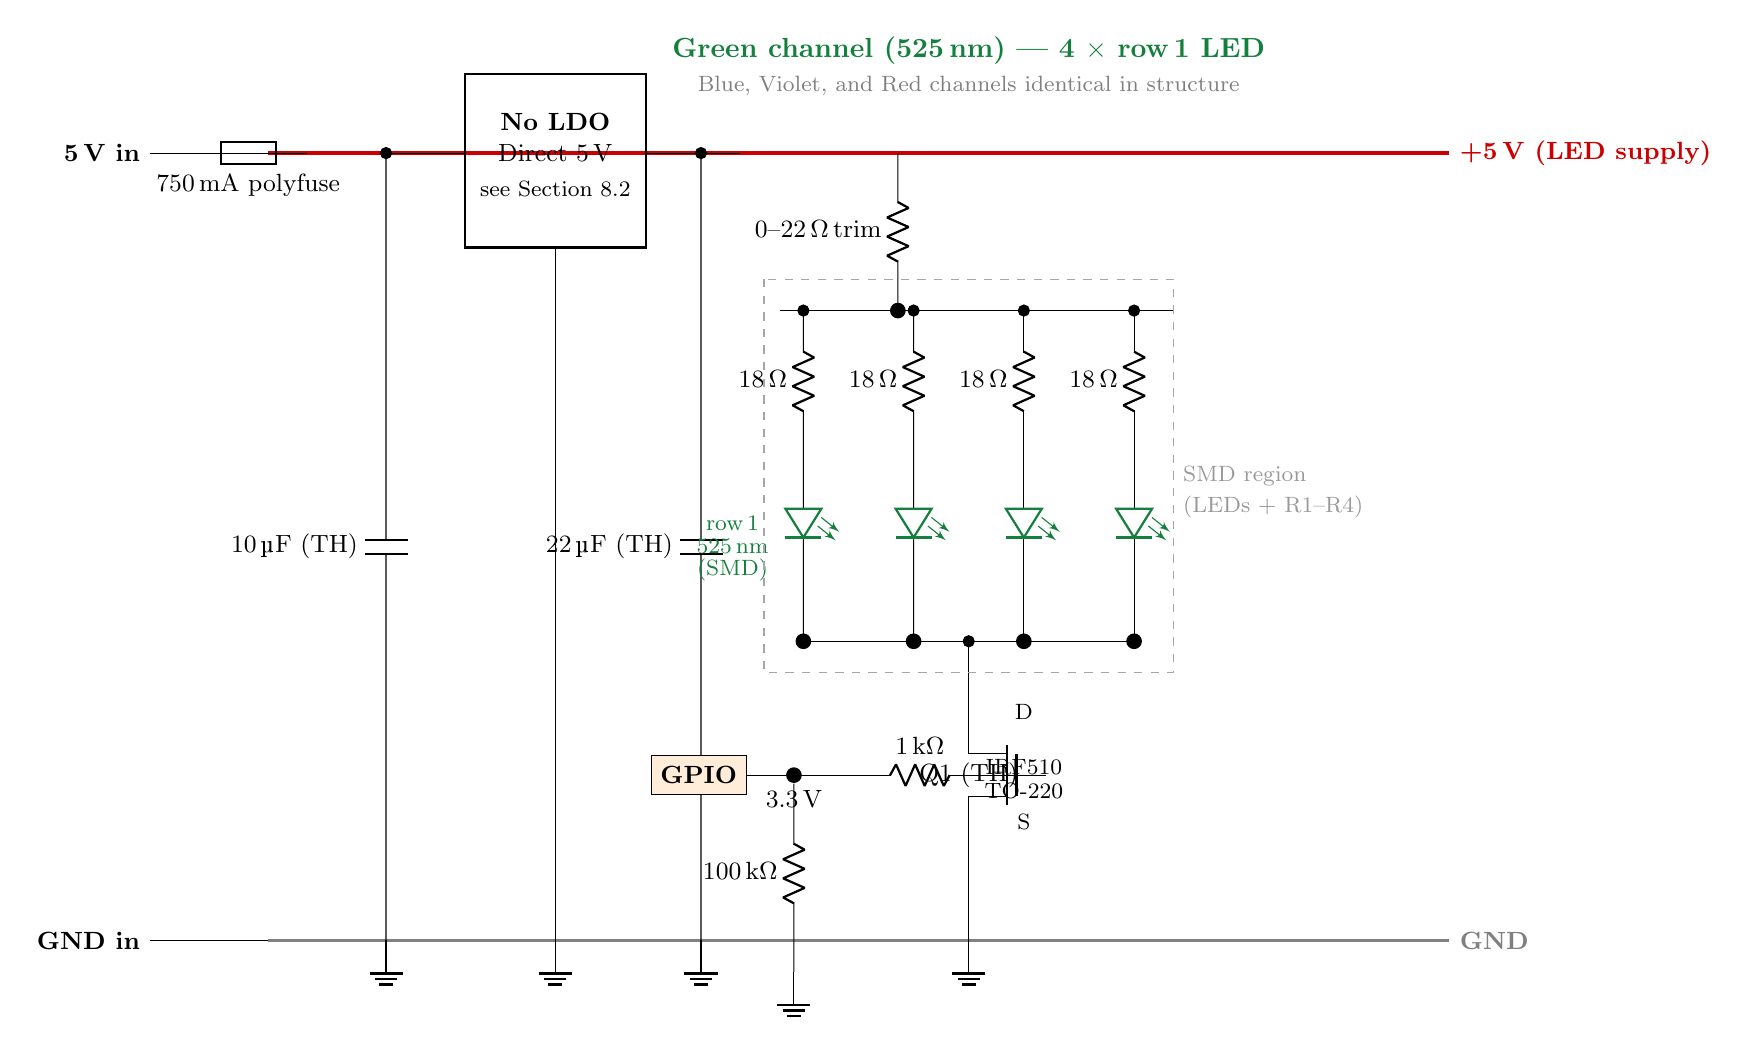
\begin{tikzpicture}[scale=1.0, transform shape,
    every node/.style={font=\small}]

\ctikzset{
  resistors/scale=0.65,
  diodes/scale=0.65,
  transistors/scale=1.0,
  capacitors/scale=0.65,
}

% ── Rails ─────────────────────────────────────────────────────────────────────
% +5V rail at y=10, GND at y=0
\draw[red!80!black, very thick] (-1, 10) -- (14, 10)
  node[right, red!80!black]{\textbf{+5\,V (LED supply)}};
\draw[black!50, very thick] (-1, 0) -- (14, 0)
  node[right, black!50]{\textbf{GND}};

% ── 5V INPUT AND POLYFUSE ─────────────────────────────────────────────────────
\draw (-2.5, 10) node[left]{\textbf{5\,V in}} to[short] (-2.0, 10);
\draw (-2.0, 10) to[fuse, l={\small PF1 (TH)}, l_={\small 750\,mA polyfuse}] (-0.5, 10);
% junction to rail
\draw (-0.5, 10) to[short] (-1, 10);
% fuse to GND (input GND)
\draw (-2.5, 0) node[left]{\textbf{GND in}} to[short] (-1, 0);

% ── LDO ───────────────────────────────────────────────────────────────────────
% LDO box between x=1..3, y=8.5..11.5 -- sits off the main rail
% Input cap (10uF) before LDO
\draw (0.5, 10) to[C, l={\small C1}, l_={\small 10\,\textmu F (TH)}] (0.5, 0);
\draw (0.5, 0) node[ground]{};
% LDO box
\draw[thick] (1.5, 8.8) rectangle (3.8, 11.0);
\node[align=center] at (2.65, 10.4) {\small\textbf{No LDO}};
\node[align=center] at (2.65, 10.0) {\small Direct 5\,V};
\node[align=center] at (2.65, 9.55) {\footnotesize see Section~8.2};
% Input wire into LDO
\draw (1.5, 10) -- (0.5, 10);
% node at LDO input
\draw[fill] (0.5,10) circle (2pt);
% Output wire from LDO
\draw (3.8, 10) -- (4.5, 10);
\draw[fill] (4.5,10) circle (2pt);
% LDO GND pin
\draw (2.65, 8.8) -- (2.65, 0);
\draw (2.65, 0) node[ground]{};
% Output cap (22uF) after LDO
\draw (4.5, 10) to[C, l={\small C2}, l_={\small 22\,\textmu F (TH)}] (4.5, 0);
\draw (4.5, 0) node[ground]{};
% connect to main rail
\draw (4.5, 10) -- (5.0, 10);

% ── LED GROUP ─────────────────────────────────────────────────────────────────
% Rshare from rail down to node A at y=8.0
\draw (7.0, 10) to[R, l={\small R\textsubscript{sh} (TH)}, l_={\small 0--22\,$\Omega$\,trim}]
  (7.0, 8.0) node[circle, fill, inner sep=2pt](NA){};

% Horizontal distribution bus from x=5.5 to x=10.5 at y=8.0
\draw (5.5, 8.0) -- (10.5, 8.0);
\draw[fill] (7.0, 8.0) circle (2pt);

% Four LED branches at x = 5.8, 7.2, 8.6, 10.0 (evenly spaced)
% Branch 1
\draw[fill] (5.8, 8.0) circle (2pt);
\draw (5.8, 8.0) to[R, l={\small R1\,(SMD)}, l_={\small 18\,$\Omega$}] (5.8, 6.2)
  to[led, color=ledgreen] (5.8, 4.4)
  -- (5.8, 3.8) node[circle, fill, inner sep=2pt](D1){};

% Branch 2
\draw[fill] (7.2, 8.0) circle (2pt);
\draw (7.2, 8.0) to[R, l={\small R2\,(SMD)}, l_={\small 18\,$\Omega$}] (7.2, 6.2)
  to[led, color=ledgreen] (7.2, 4.4)
  -- (7.2, 3.8) node[circle, fill, inner sep=2pt](D2){};

% Branch 3
\draw[fill] (8.6, 8.0) circle (2pt);
\draw (8.6, 8.0) to[R, l={\small R3\,(SMD)}, l_={\small 18\,$\Omega$}] (8.6, 6.2)
  to[led, color=ledgreen] (8.6, 4.4)
  -- (8.6, 3.8) node[circle, fill, inner sep=2pt](D3){};

% Branch 4
\draw[fill] (10.0, 8.0) circle (2pt);
\draw (10.0, 8.0) to[R, l={\small R4\,(SMD)}, l_={\small 18\,$\Omega$}] (10.0, 6.2)
  to[led, color=ledgreen] (10.0, 4.4)
  -- (10.0, 3.8) node[circle, fill, inner sep=2pt](D4){};

% LED labels between resistor and LED on branch 1
\node[ledgreen, font=\footnotesize] at (4.9, 5.3) {row\,1};
\node[ledgreen, font=\footnotesize] at (4.9, 5.0) {525\,nm};
\node[ledgreen, font=\footnotesize] at (4.9, 4.7) {(SMD)};

% Cathode bus at y=3.8
\draw (5.8, 3.8) -- (10.0, 3.8);
% Drop to drain node at x=7.9, y=3.8 then down to MOSFET
\draw[fill] (7.9, 3.8) circle (2pt);
\draw (7.9, 3.8) -- (7.9, 3.0);

% ── MOSFET ───────────────────────────────────────────────────────────────────
% MOSFET drain at (7.9, 3.0), source at (7.9, 1.2)
% Using Tnmos which places gate to the left
\draw (7.9, 3.0) to[Tnmos, n=QG, l={\small Q1 (TH)}] (7.9, 1.2);
\draw (7.9, 1.2) -- (7.9, 0) node[ground]{};
% Drain/Source labels
\node[font=\footnotesize] at (8.6, 2.9) {D};
\node[font=\footnotesize] at (8.6, 1.5) {S};
\node[font=\footnotesize] at (8.6, 2.2) {IRF510};
\node[font=\footnotesize] at (8.6, 1.9) {TO-220};

% ── GATE CIRCUIT ─────────────────────────────────────────────────────────────
% Gate node from MOSFET goes left
% Gate of QG is at QG.gate
% Draw gate resistor from gate leftward to GPIO node
\draw (QG.gate) to[R, l={\small Rg (TH)}, l_={\small 1\,k$\Omega$}] ++(-3.2, 0)
  node[circle, fill, inner sep=2pt](GPIN){};

% Pull-down from GPIN to ground
\draw (GPIN) to[R, l_={\small R\textsubscript{pd} (TH)}, l={\small 100\,k$\Omega$}]
  ++(0, -2.5) node[ground]{};

% GPIO input label with box
\draw (GPIN) -- ++(-0.6, 0)
  node[draw, rectangle, minimum width=1.1cm, minimum height=0.5cm,
       fill=orange!15, font=\small\bfseries, left]{\small GPIO};
\node[font=\footnotesize, below=2pt] at (GPIN) {\small 3.3\,V};

% ── GROUP LABEL ───────────────────────────────────────────────────────────────
\node[ledgreen, font=\bfseries] at (7.9, 11.3)
  {Green channel (525\,nm) --- 4 $\times$ row\,1 LED};
\node[font=\footnotesize, gray] at (7.9, 10.85)
  {Blue, Violet, and Red channels identical in structure};

% ── ANNOTATION LINES ──────────────────────────────────────────────────────────
% SMD region brace annotation
\draw[dashed, gray!70] (5.3, 8.4) rectangle (10.5, 3.4);
\node[gray!80, font=\footnotesize, right] at (10.5, 5.9) {SMD region};
\node[gray!80, font=\footnotesize, right] at (10.5, 5.5) {(LEDs + R1--R4)};

\end{tikzpicture}
\caption{Single LED driver channel (green group, 4 LEDs shown). The dashed box encloses
the SMD components: the four LEDs (row~1, 1411 package) and their individual 18~\si{\ohm}
current-setting resistors. All other components are through-hole (TH). The polyfuse (PF1)
and LDO with input/output capacitors (C1, C2) are shared across all four color channels.
The gate resistor (Rg) and pull-down ($R_{pd}$) protect the MOSFET gate from the GPIO.
Blue, violet, and red channels use the same circuit with different LED parts and resistor values.}
\label{fig:schematic}
\end{figure}

% ═════════════════════════════════════════════════════════════════════════════
\section{Key Calculations}
% ═════════════════════════════════════════════════════════════════════════════

\subsection{LED Current and Ohm's Law}

The current through each LED is controlled by its individual series resistor.
The voltage across the resistor is the supply voltage minus the LED's forward voltage drop:

\begin{equation}
  V_R = V_{CC} - V_f
  \label{eq:vr}
\end{equation}

By Ohm's law, the current through the resistor (and LED) is:

\begin{equation}
  I_{LED} = \frac{V_R}{R} = \frac{V_{CC} - V_f}{R}
  \label{eq:iled}
\end{equation}

Rearranging to find the resistor value for a desired current:

\begin{equation}
  R = \frac{V_{CC} - V_f}{I_{LED}}
  \label{eq:r}
\end{equation}

\subsection{Power Dissipation in the Resistor}

The power dissipated as heat in the resistor is:

\begin{equation}
  P_R = I_{LED}^2 \times R
  \label{eq:pr}
\end{equation}

This is important for choosing the correct resistor physical size (power rating).

\subsection{Total Group Current}

Since all $N$ LEDs in a group are in parallel, the total current drawn from the supply
when one group is active is:

\begin{equation}
  I_{total} = N \times I_{LED}
  \label{eq:itotal}
\end{equation}

This total current must not exceed the 500\,mA budget.

\subsection{Brightness Levels}

Three brightness levels are defined as fractions of the LED's maximum rated current
($I_{max}$):

\begin{itemize}[leftmargin=2em]
  \item \textbf{Low:} $I_{LED} \approx 40\%$ of $I_{max}$
  \item \textbf{Medium:} $I_{LED} \approx 60\%$ of $I_{max}$ (preferred operating point)
  \item \textbf{High:} $I_{LED} \approx 80\%$ of $I_{max}$ (or constrained by budget)
\end{itemize}

The Medium level targets the range of 50--75\% of $I_{max}$, balancing good brightness,
reasonable LED lifetime, and staying within the power budget.

% ═════════════════════════════════════════════════════════════════════════════
\section{Sample Calculation: Green LED (Row~1, Medium Level)}
% ═════════════════════════════════════════════════════════════════════════════

This section works through a complete calculation for the first-choice green LED,
row~1 (525\,nm, 1411 package, \$0.23 each), at the Medium brightness level.
All other LEDs in the table follow the same procedure.

\textbf{Given:}
\begin{itemize}[leftmargin=2em]
  \item Supply voltage: $V_{CC} = 5.0$\,V
  \item LED forward voltage: $V_f = 2.80$\,V (typical)
  \item LED maximum current: $I_{max} = 240$\,mA
  \item Number of LEDs: $N = 4$
  \item Target level: Medium = 62.5\% of $I_{max}$
\end{itemize}

\textbf{Step 1: Target current per LED}
\[
  I_{target} = 0.625 \times 240\,\text{mA} = 150\,\text{mA}
\]

\textbf{Step 2: Check total group current}
\[
  I_{total} = 4 \times 150\,\text{mA} = 600\,\text{mA}
\]
This exceeds the 500\,mA budget, so the target must be reduced.
At 500\,mA budget with 4 LEDs: $I_{LED,\max} = 500/4 = 125$\,mA.
Use $I_{target} = 122$\,mA (50.9\% of $I_{max}$, acceptable).

\textbf{Step 3: Calculate resistor value}
\[
  R = \frac{V_{CC} - V_f}{I_{target}} = \frac{5.0 - 2.80}{0.122} = \frac{2.20}{0.122} \approx 18.0\,\Omega
\]

\textbf{Step 4: Select nearest E24 standard value}\\
The E24 series includes 18\,\si{\ohm} exactly. Use \textbf{18\,\si{\ohm}}.

\textbf{Step 5: Confirm actual current with the standard resistor}
\[
  I_{actual} = \frac{5.0 - 2.80}{18} = \frac{2.20}{18} = 122.2\,\text{mA per LED}
\]
\[
  I_{total} = 4 \times 122.2 = 488.9\,\text{mA} \quad \text{(within 500\,mA budget)}
\]

\textbf{Step 6: Calculate resistor power dissipation}
\[
  P_R = I^2 \times R = (0.1222)^2 \times 18 = 0.01493 \times 18 \approx 0.27\,\text{W}
\]
A standard 0603 SMD resistor is rated 0.1\,W and would fail.
An \textbf{0805 (0.25\,W)} is marginal; a \textbf{1206 (0.25--0.5\,W)} is the safe choice.

\textbf{Step 7: Power in the LED}
\[
  P_{LED} = V_f \times I_{actual} = 2.80 \times 0.1222 \approx 342\,\text{mW per LED}
\]
\[
  P_{group} = 4 \times 342 = 1.37\,\text{W total in LEDs}
\]

The LEDs are in 3528 packages with a copper pad on the PCB; they will run warm but
within safe limits at this power level.

% ═════════════════════════════════════════════════════════════════════════════
\section{Candidate LED Table}
% ═════════════════════════════════════════════════════════════════════════════

Table~\ref{tab:candidates} lists the top three candidate LEDs for each color channel,
selected from the supplier catalog based on wavelength, price, package, viewing angle,
and availability ($\geq$1 unit, active status).

\renewcommand{\arraystretch}{1.3}
\begin{table}[H]
\centering
\small
\caption{Top three LED candidates per color channel}
\label{tab:candidates}
\begin{tabular}{C{0.4cm} L{1.0cm} C{0.5cm} C{1.3cm} C{1.1cm} C{1.0cm} C{1.0cm} C{1.5cm} C{1.3cm} C{0.7cm}}
\toprule
\# & \textbf{Color} & \textbf{Rnk} & \textbf{Wavelength} & \textbf{Package} & $V_f$ & $I_{max}$ & \textbf{Flux} & \textbf{Angle} & \textbf{Price} \\
\midrule
\rowcolor{lightviolet}
1015 & Violet & 1 & 410\,nm dom & 0603 & 2.80\,V & $\sim$30\,mA† & --- & 130° & \$0.42 \\
\rowcolor{lightviolet}
1012 & Violet & 2 & 455\,nm dom & 1411 & 3.00\,V & $\sim$100\,mA† & 850\,mcd & 120° & \$0.29 \\
\rowcolor{lightviolet}
4    & Violet & 3 & 455\,nm     & 1411 & 2.96\,V & 240\,mA & 265\,mW & 124° & \$0.26 \\
\midrule
\rowcolor{lightblue}
2    & Blue   & 1 & 475\,nm     & 1411 & 2.95\,V & 240\,mA & 20\,lm & 126° & \$0.24 \\
\rowcolor{lightblue}
1014 & Blue   & 2 & 455\,nm dom & 4-SMD & 3.20\,V & $\sim$200\,mA† & 2100\,mcd & 120° & \$0.40 \\
\rowcolor{lightblue}
102  & Blue   & 3 & 465\,nm     & 1411 & 3.20\,V & 200\,mA & 11\,lm & 120° & \$0.32 \\
\midrule
\rowcolor{lightgreen}
1    & Green  & 1 & 525\,nm     & 1411 & 2.80\,V & 240\,mA & 62\,lm & 124° & \$0.23 \\
\rowcolor{lightgreen}
532  & Green  & 2 & 525\,nm dom & 1411 & 3.10\,V & $\sim$30\,mA† & 1000\,mcd & 120° & \$0.19 \\
\rowcolor{lightgreen}
783  & Green  & 3 & 525\,nm dom & 1411 & 3.40\,V & $\sim$200\,mA† & 8000\,mcd & 120° & \$0.36 \\
\midrule
\rowcolor{lightred}
3    & Red    & 1 & 625\,nm     & 1411 & 2.20\,V & 250\,mA & 26\,lm & 122° & \$0.26 \\
\rowcolor{lightred}
727  & Red    & 2 & 624\,nm dom & 1411 & 2.00\,V & $\sim$200\,mA† & 4500\,mcd & 120° & \$0.33 \\
\rowcolor{lightred}
6    & Red    & 3 & 620\,nm     & 1411 & 2.20\,V & 200\,mA & 24\,lm & 120° & \$0.32 \\
\bottomrule
\end{tabular}\\[4pt]
\raggedright\footnotesize † $I_{max}$ estimated; no datasheet value available. Treat conservatively.
\end{table}

% ═════════════════════════════════════════════════════════════════════════════
\section{Resistor Value Table}
% ═════════════════════════════════════════════════════════════════════════════

Table~\ref{tab:resistors} gives the E24 standard resistor value for each LED option
at Low, Medium, and High brightness, along with the resulting actual current and
total group current. Entries marked \textcolor{warnred}{\textbf{OVER}} exceed the
500\,mA budget and should not be used without a higher-rated power supply or
fewer LEDs. Estimated $I_{max}$ values are marked with $\dagger$.

\renewcommand{\arraystretch}{1.25}
\begin{longtable}{C{0.6cm} L{1.0cm} C{0.5cm} C{0.5cm} C{1.0cm} C{0.8cm} C{0.9cm}
                  C{1.1cm} C{1.1cm} C{0.9cm} C{0.9cm} C{0.9cm}}
\caption{Resistor values for all LED options and brightness levels ($V_{CC} = 5.0$\,V, $R_{share} = 0\,\Omega$)}
\label{tab:resistors}\\
\toprule
\textbf{Row} & \textbf{Color} & \textbf{Rnk} & \textbf{N} & \textbf{Level} &
$V_f$ & $I_{max}$ & \textbf{R E24} & $I_{act}$ & $I_{tot}$ & \%$I_{max}$ & \textbf{Notes} \\
 & & & & & (V) & (mA) & (\si{\ohm}) & (mA) & (mA) & & \\
\midrule
\endfirsthead
\multicolumn{12}{l}{\small\itshape Table~\ref{tab:resistors} continued\ldots}\\
\toprule
\textbf{Row} & \textbf{Color} & \textbf{Rnk} & \textbf{N} & \textbf{Level} &
$V_f$ & $I_{max}$ & \textbf{R E24} & $I_{act}$ & $I_{tot}$ & \%$I_{max}$ & \textbf{Notes} \\
\midrule
\endhead
\bottomrule
\endfoot

% Violet rows
\rowcolor{lightviolet}
1015 & Violet & 1 & 4 & Low  & 2.80 & 30† & 180 & 12.2 & 49  & 41\% & \\
\rowcolor{lightviolet}
1015 & Violet & 1 & 4 & \textbf{Med}  & 2.80 & 30† & \textbf{120} & 18.3 & 73  & 61\% & \\
\rowcolor{lightviolet}
1015 & Violet & 1 & 4 & High & 2.80 & 30† & 82  & 26.8 & 107 & 89\% & Near limit \\
\rowcolor{lightviolet}
1015 & Violet & 1 & 6 & Low  & 2.80 & 30† & 180 & 12.2 & 73  & 41\% & \\
\rowcolor{lightviolet}
1015 & Violet & 1 & 6 & \textbf{Med}  & 2.80 & 30† & \textbf{120} & 18.3 & 110 & 61\% & \\
\rowcolor{lightviolet}
1015 & Violet & 1 & 6 & High & 2.80 & 30† & 82  & 26.8 & 161 & 89\% & Near limit \\
\rowcolor{lightviolet}
1012 & Violet & 2 & 4 & Low  & 3.00 & 100† & 51 & 39.2 & 157 & 39\% & \\
\rowcolor{lightviolet}
1012 & Violet & 2 & 4 & \textbf{Med}  & 3.00 & 100† & \textbf{33} & 60.6 & 242 & 61\% & \\
\rowcolor{lightviolet}
1012 & Violet & 2 & 4 & High & 3.00 & 100† & 24  & 83.3 & 333 & 83\% & \\
\rowcolor{lightviolet}
1012 & Violet & 2 & 6 & Low  & 3.00 & 100† & 51  & 39.2 & 235 & 39\% & \\
\rowcolor{lightviolet}
1012 & Violet & 2 & 6 & \textbf{Med}  & 3.00 & 100† & \textbf{33} & 60.6 & 364 & 61\% & \\
\rowcolor{lightviolet}
1012 & Violet & 2 & 6 & High & 3.00 & 100† & 24  & 83.3 & 500 & 83\% & At limit \\
\rowcolor{lightviolet}
4    & Violet & 3 & 4 & Low  & 2.96 & 240 & 39  & 52.3 & 209 & 22\% & Below 50\% \\
\rowcolor{lightviolet}
4    & Violet & 3 & 4 & \textbf{Med}  & 2.96 & 240 & \textbf{24} & 85.0 & 340 & 35\% & Below 50\% \\
\rowcolor{lightviolet}
4    & Violet & 3 & 4 & High & 2.96 & 240 & 18  & 113.3 & 453 & 47\% & Below 50\% \\
\rowcolor{lightviolet}
4    & Violet & 3 & 6 & Low  & 2.96 & 240 & 39  & 52.3 & 314 & 22\% & \\
\rowcolor{lightviolet}
4    & Violet & 3 & 6 & \textbf{Med}  & 2.96 & 240 & \textbf{24} & 85.0 & \textcolor{warnred}{\textbf{510}} & 35\% & \textcolor{warnred}{OVER} \\
\rowcolor{lightviolet}
4    & Violet & 3 & 6 & High & 2.96 & 240 & 18  & 113.3 & \textcolor{warnred}{\textbf{680}} & 47\% & \textcolor{warnred}{OVER} \\
\midrule
% Blue rows
\rowcolor{lightblue}
2    & Blue   & 1 & 4 & Low  & 2.95 & 240 & 27  & 75.9 & 304 & 32\% & \\
\rowcolor{lightblue}
2    & Blue   & 1 & 4 & \textbf{Med}  & 2.95 & 240 & \textbf{18} & 113.9 & 455 & 47\% & \\
\rowcolor{lightblue}
2    & Blue   & 1 & 4 & High & 2.95 & 240 & 15  & 136.7 & \textcolor{warnred}{\textbf{547}} & 57\% & \textcolor{warnred}{OVER} \\
\rowcolor{lightblue}
1014 & Blue   & 2 & 4 & Low  & 3.20 & 200† & 22 & 81.8 & 327 & 41\% & \\
\rowcolor{lightblue}
1014 & Blue   & 2 & 4 & \textbf{Med}  & 3.20 & 200† & \textbf{15} & 120.0 & 480 & 60\% & \\
\rowcolor{lightblue}
1014 & Blue   & 2 & 4 & High & 3.20 & 200† & 15  & 120.0 & 480 & 60\% & Same R as Med \\
\rowcolor{lightblue}
102  & Blue   & 3 & 4 & Low  & 3.20 & 200 & 27  & 66.7 & 267 & 33\% & \\
\rowcolor{lightblue}
102  & Blue   & 3 & 4 & \textbf{Med}  & 3.20 & 200 & \textbf{15} & 120.0 & 480 & 60\% & \\
\rowcolor{lightblue}
102  & Blue   & 3 & 4 & High & 3.20 & 200 & 11  & 163.6 & \textcolor{warnred}{\textbf{655}} & 82\% & \textcolor{warnred}{OVER} \\
\midrule
% Green rows
\rowcolor{lightgreen}
1    & Green  & 1 & 4 & Low  & 2.80 & 240 & 30  & 73.3 & 293 & 31\% & \\
\rowcolor{lightgreen}
1    & Green  & 1 & 4 & \textbf{Med}  & 2.80 & 240 & \textbf{18} & 122.2 & 489 & 51\% & \\
\rowcolor{lightgreen}
1    & Green  & 1 & 4 & High & 2.80 & 240 & 15  & 146.7 & \textcolor{warnred}{\textbf{587}} & 61\% & \textcolor{warnred}{OVER} \\
\rowcolor{lightgreen}
532  & Green  & 2 & 4 & Low  & 3.10 & 30† & 160 & 11.9 & 48  & 40\% & \\
\rowcolor{lightgreen}
532  & Green  & 2 & 4 & \textbf{Med}  & 3.10 & 30† & \textbf{100} & 19.0 & 76  & 63\% & \\
\rowcolor{lightgreen}
532  & Green  & 2 & 4 & High & 3.10 & 30† & 75  & 25.3 & 101 & 84\% & Near limit \\
\rowcolor{lightgreen}
783  & Green  & 3 & 4 & Low  & 3.40 & 200† & 20 & 80.0 & 320 & 40\% & \\
\rowcolor{lightgreen}
783  & Green  & 3 & 4 & \textbf{Med}  & 3.40 & 200† & \textbf{13} & 123.1 & 492 & 62\% & \\
\rowcolor{lightgreen}
783  & Green  & 3 & 4 & High & 3.40 & 200† & 13  & 123.1 & 492 & 62\% & Same R as Med \\
\midrule
% Red rows
\rowcolor{lightred}
3    & Red    & 1 & 4 & Low  & 2.20 & 250 & 36  & 77.8 & 311 & 31\% & \\
\rowcolor{lightred}
3    & Red    & 1 & 4 & \textbf{Med}  & 2.20 & 250 & \textbf{24} & 116.7 & 467 & 47\% & Use 24\,\si{\ohm} \\
\rowcolor{lightred}
3    & Red    & 1 & 4 & High & 2.20 & 250 & 20  & 140.0 & \textcolor{warnred}{\textbf{560}} & 56\% & \textcolor{warnred}{OVER} \\
\rowcolor{lightred}
727  & Red    & 2 & 4 & Low  & 2.00 & 200† & 36 & 83.3 & 333 & 42\% & \\
\rowcolor{lightred}
727  & Red    & 2 & 4 & \textbf{Med}  & 2.00 & 200† & \textbf{24} & 125.0 & 500 & 63\% & At limit \\
\rowcolor{lightred}
727  & Red    & 2 & 4 & High & 2.00 & 200† & 18  & 166.7 & \textcolor{warnred}{\textbf{667}} & 83\% & \textcolor{warnred}{OVER} \\
\rowcolor{lightred}
6    & Red    & 3 & 4 & Low  & 2.20 & 200 & 39  & 71.8 & 287 & 36\% & \\
\rowcolor{lightred}
6    & Red    & 3 & 4 & \textbf{Med}  & 2.20 & 200 & \textbf{24} & 116.7 & 467 & 58\% & \\
\rowcolor{lightred}
6    & Red    & 3 & 4 & High & 2.20 & 200 & 22  & 127.3 & \textcolor{warnred}{\textbf{509}} & 64\% & \textcolor{warnred}{OVER} \\

\end{longtable}

% ═════════════════════════════════════════════════════════════════════════════
\section{Design Decisions and Explanations}
% ═════════════════════════════════════════════════════════════════════════════

\subsection{First-Choice LEDs at Medium Brightness}

The recommended build uses the first-choice LED for each color at Medium brightness:

\begin{center}
\renewcommand{\arraystretch}{1.3}
\begin{tabular}{L{1.5cm} C{0.8cm} C{0.5cm} C{1.5cm} C{1.3cm} C{1.3cm} C{1.3cm}}
\toprule
\textbf{Channel} & \textbf{Row} & \textbf{N} & \textbf{R (\si{\ohm})} & $I$/LED & $I_{total}$ & \textbf{Price/LED} \\
\midrule
\rowcolor{lightviolet} Violet & 1015 & 6 & 120 & 18\,mA & 110\,mA & \$0.42 \\
\rowcolor{lightblue}   Blue   & 2    & 4 & 18  & 114\,mA & 455\,mA & \$0.24 \\
\rowcolor{lightgreen}  Green  & 1    & 4 & 18  & 122\,mA & 489\,mA & \$0.23 \\
\rowcolor{lightred}    Red    & 3    & 4 & 24  & 117\,mA & 467\,mA & \$0.26 \\
\bottomrule
\end{tabular}
\end{center}

All four first-choice LEDs share the \textbf{1411 (3528) package}, simplifying PCB layout.
The total cost for 18 LEDs (6 violet + 4 each of blue, green, red) is approximately \$5.

\textbf{Why Medium, not High?} The Medium level keeps all groups except blue below 490\,mA,
within the 500\,mA budget. More importantly, operating at 50--65\% of rated current significantly
extends LED lifetime and keeps junction temperatures low, which is good for long-term
measurement stability---thermal drift in LEDs changes their output spectrum slightly.

\textbf{Exposure time as the fine-tuning knob.} Because the camera can vary exposure from
a short flash to 1.2\,seconds, the resistors set a fixed hardware brightness and the software
adjusts exposure to hit the right sensor reading. This is more repeatable than varying the LED
current in software.

\subsection{The Violet Channel Caveat}

Row~1015 is the only true violet/near-UV LED in the catalog (410\,nm). Its datasheet provides
no maximum current figure, which is unusual. The LED is in a 0603 package (1.6\,mm $\times$
0.8\,mm) --- a small indicator device. Based on comparable 0603 indicator LEDs from other
manufacturers, 30\,mA is a conservative estimate.

At Medium brightness (120\,\si{\ohm}, 18\,mA per LED, 110\,mA total for 6 LEDs) the device
is well within any plausible limit. The High setting approaches the estimated limit and should
only be used briefly for testing while monitoring LED temperature.

\subsection{Why Row~4 (Power LED Violet) Was Downgraded}

Row~4 is a high-power 455\,nm LED (240\,mA rated). Even though it is brighter, the power
budget constrains it to well below 50\% of its rated current---it is simply too large a device
for this application. Row~1015 at 410\,nm is a better wavelength choice and a more appropriate
size.

\subsection{Individual Resistors and the Shared Trim Resistor}

LEDs of the same type from the same reel can have $V_f$ variations of $\pm$0.1--0.2\,V.
On a 5\,V supply with an 18\,\si{\ohm} resistor, a 0.1\,V variation in $V_f$ changes the
LED current by $0.1/18 \approx 5.6$\,mA --- a small, tolerable variation. Individual resistors
ensure each LED is independently current-controlled regardless of its $V_f$.

The optional shared series resistor ($R_{share}$, 0--22\,\si{\ohm}) trims the entire group's
brightness uniformly. Start with a wire (0\,\si{\ohm}). If the camera saturates on any channel
at Medium brightness, add a resistor here rather than changing all four individual resistors.
A 10\,\si{\ohm} potentiometer temporarily installed during commissioning lets you find the
right value, which you then replace with a fixed resistor.

% ═════════════════════════════════════════════════════════════════════════════
\section{Interesting Remarks}
% ═════════════════════════════════════════════════════════════════════════════

\subsection{Channel Separation Is Excellent}

The four selected wavelengths --- 410, 475, 525, and 625\,nm --- are well separated across
the visible spectrum. The gaps are 65\,nm, 50\,nm, and 100\,nm respectively. The camera's
RGB Bayer filter will respond differently to each channel, and the color algorithm can
exploit this differential response to extract significantly more spectral information than
a white-light photograph provides.

\subsection{Green LEDs Are Disproportionately Bright}

The human eye (and most camera sensors) are most sensitive to green light. Row~1,
the first-choice green LED, produces 62\,lm at 140\,mA --- roughly 2.4$\times$ the flux
of the red LED and far more than the blue. Even at Medium brightness (122\,mA),
this is a bright green emitter. If green overexposes the camera at medium brightness
and a short exposure, use the Low setting (30\,\si{\ohm}) or add a small $R_{share}$.

\subsection{The Violet LED: Confirmed Specs, Wide Voltage Tolerance}

Row~1015 is now confirmed from its datasheet: absolute maximum current 30~mA,
maximum power dissipation 120~mW, $V_f$ ranging from 2.8~V (minimum/typical) to
4.0~V (maximum). The wide forward voltage tolerance deserves attention.

At worst-case $V_f = 4.0$~V on a 5~V supply, the resistor only sees 1.0~V.
With the 120~\si{\ohm} current-setting resistor this gives $1.0/120 = 8.3$~mA.
At the typical $V_f = 2.8$~V the same resistor gives $(5.0-2.8)/120 = 18.3$~mA.
LEDs from the same reel may therefore span roughly 8--18~mA and vary in brightness.
This is acceptable for this application because the camera exposure time compensates
for overall group brightness; within the group, the brighter LEDs simply have a lower $V_f$.

The 120~mW dissipation limit is consistent: $4.0~\text{V} \times 30~\text{mA} = 120~\text{mW}$.
Operating at 18~mA with a typical $V_f$ of 2.8~V gives $2.8 \times 0.0183 = 51$~mW per LED,
well within limits. All six LEDs together draw only 110~mA --- by far the lightest load
of the four channels.

\subsection{Resistor Power Ratings Are Easy to Overlook}

This is the most common mistake in LED driver design. A 120\,\si{\ohm} resistor at
18\,mA dissipates only $0.018^2 \times 120 = 39$\,mW --- a 0402 can handle this.
But an 18\,\si{\ohm} resistor at 122\,mA dissipates 268\,mW --- a standard 0603
will get hot enough to change value or fail. Always calculate resistor dissipation
and check the datasheet power rating for your package size.

\subsection{The 500\,mA Budget Is Actually Generous for This Application}

The LEDs fire one group at a time, and exposures can be as short as a fraction of a
second. The average power draw is far lower than the 500\,mA peak. The LDO regulator
and polyfuse are sized for the worst-case peak; in normal operation the system will
draw 100--500\,mA for brief intervals separated by longer idle periods.

% ═════════════════════════════════════════════════════════════════════════════
\section{Recommended Supporting Components}
% ═════════════════════════════════════════════════════════════════════════════

\subsection{MOSFET: IRL540N or IRFZ44N (Through-Hole, TO-220)}

Since through-hole assembly is preferred for all non-LED components, the MOSFET
selection moves to TO-220 power packages. These are large, robust, easy to hand-solder,
and available from any general electronics supplier.

\textbf{Why not the 2N7000?} The 2N7000 is a TO-92 through-hole part but rated at only
200~mA drain current --- insufficient for the blue and green groups at medium brightness
(455--489~mA). Do not use it for this circuit.

Recommended parts:

\begin{center}
\begin{tabular}{lll}
\toprule
\textbf{Parameter} & \textbf{IRL540N} & \textbf{IRFZ44N} \\
\midrule
Maximum drain current ($I_D$) & 36\,A & 49\,A \\
On-resistance ($R_{DS(on)}$) & 0.077\,\si{\ohm} at $V_{GS}=10$\,V & 0.017\,\si{\ohm} at $V_{GS}=10$\,V \\
Gate threshold (max) & 2.0\,V & 4.0\,V \\
Logic-level (3.3\,V GPIO) & Yes --- fully on & Partially on; see note \\
Package & TO-220 & TO-220 \\
Approximate price & \$0.80--1.20 & \$0.50--0.80 \\
\bottomrule
\end{tabular}
\end{center}

\textbf{Recommended choice: IRL540N.} It is a true logic-level device with gate threshold
$\leq$2~V, guaranteed to switch fully on from a 3.3~V GPIO. At 500~mA the on-resistance
causes a drop of only $0.5 \times 0.077 = 39$~mV and dissipates $0.5^2 \times 0.077 = 19$~mW
--- the TO-220 package needs no heatsink.

The \textbf{IRFZ44N} is cheaper and widely available but its threshold can be up to 4~V,
so it may not switch fully on at 3.3~V. It will work well enough for this low-duty-cycle
application (LEDs fire briefly for a photograph) but the IRL540N is cleaner.

\subsection{LDO Voltage Regulator: Not Used --- Direct 5\,V Connection}

\textbf{The supply voltage is exactly 5\,V, which rules out any linear voltage regulator
for the LED rail.}

A linear regulator (LDO or otherwise) requires its input to be \emph{higher} than its
output by at least the dropout voltage. For the LD1117, dropout is $\approx 1.2$\,V,
requiring at least 6.2\,V in to deliver 5.0\,V out. Even the best ultra-low-dropout
regulators (e.g.\ MCP1700, $V_{dropout} \approx 0.18$\,V at 250\,mA) need $\geq$5.18\,V
input --- still more than 5.0\,V. There is no linear regulator that can produce 5.0\,V
from a 5.0\,V input; the output will always be lower than the input by at least the
dropout, and the regulator will fall out of regulation.

\textbf{What to do instead:} Connect the LED circuit directly to the 5\,V supply rail
(after the polyfuse), and use bulk decoupling capacitors to handle the current transients
when each LED group switches on. The goal of isolating the LED load from the Pi's logic
supply is achieved by routing them as separate branches from the main 5\,V connector,
and by the impedance of the polyfuse and PCB traces acting as natural isolation.

The capacitors described in the next section take on increased importance in this
arrangement, as they are the only local energy reservoir for the LED groups.

\textbf{If a regulated LED supply is still desired} (for example, to make LED brightness
independent of supply voltage variations), the correct solution is a \textbf{switching
buck converter} that accepts 5\,V in and outputs a lower voltage, e.g.\ 3.3\,V, and
then recalculate the resistor values for that lower rail. However, this adds circuit
complexity and is not necessary for this application, where software exposure-time
calibration handles any supply variation.

\subsection{Bypass Capacitors (Through-Hole)}

Capacitors placed close to the LDO stabilize the output voltage when a LED group
switches on suddenly. Through-hole electrolytic or ceramic radial capacitors are used.

\begin{center}
\begin{tabular}{llll}
\toprule
\textbf{Ref} & \textbf{Location} & \textbf{Value} & \textbf{Type (TH)} \\
\midrule
C1 & 5\,V supply input & 100\,\si{\micro F} / 10\,V & Electrolytic radial --- bulk reservoir \\
C2 & 5\,V supply input & 100\,nF & Ceramic disc --- high-frequency bypass \\
C3--C6 & Near each LED group & 10\,\si{\micro F} / 10\,V & Electrolytic radial \\
\bottomrule
\end{tabular}
\end{center}

Since there is no LDO, the bypass capacitors become the sole transient energy reserve
for the LED groups. A larger bulk capacitor (100~\si{\micro F}) at the supply input
absorbs the current spike when each group switches on, preventing the 5\,V rail from
drooping and potentially disrupting the Raspberry Pi. The 100\,nF ceramic capacitor
handles higher-frequency noise. The 10~\si{\micro F} capacitors near each LED group
provide local charge storage close to the load where it is most effective.

Use at least 10\,V voltage rating for all capacitors on a 5\,V circuit.
Through-hole electrolytic capacitors (e.g.\ Panasonic FR or Nichicon UPW series) are
inexpensive and easy to source for the larger values; a ceramic disc is fine for the
100\,nF bypass.

\subsection{Polyfuse (Through-Hole Radial)}

A polyfuse is a thermally sensitive resistor that trips when current exceeds its rating,
protecting the supply from a short circuit. It resets automatically when it cools down.

\begin{center}
\begin{tabular}{ll}
\toprule
\textbf{Parameter} & \textbf{Value} \\
\midrule
Hold current ($I_H$) & $\geq$500\,mA \\
Trip current ($I_T$) & $\leq$1.0\,A \\
Maximum voltage & $\geq$6\,V \\
Package & Radial through-hole \\
\bottomrule
\end{tabular}
\end{center}

\textbf{Suggested parts (through-hole radial):}
\begin{itemize}[leftmargin=2em]
  \item \textbf{Bourns MF-R050} (hold 500\,mA, trip 1.0\,A, radial TH, $\sim$\$0.25)
  \item \textbf{Littelfuse 16R050} (hold 500\,mA, radial TH, $\sim$\$0.30)
  \item \textbf{TE Connectivity RXEF050} (hold 500\,mA, trip 1.0\,A, radial TH, $\sim$\$0.30)
\end{itemize}

Place the polyfuse in series with the 5\,V line going into the LDO input, as shown in
the schematic. It should be the first component in the circuit after the power connector.

\subsection{Gate and Pull-Down Resistors (Through-Hole)}

Standard through-hole 1/4\,W metal film resistors are ideal here. They are cheap, easy
to solder, and handle the tiny dissipation in the gate circuit with enormous margin.

\begin{center}
\begin{tabular}{llll}
\toprule
\textbf{Component} & \textbf{Value} & \textbf{Power} & \textbf{Function} \\
\midrule
Gate resistor ($R_g$) $\times 4$ & 1\,k\si{\ohm} & $<$1\,mW & Limits gate charge current \\
Pull-down ($R_{pd}$) $\times 4$ & 100\,k\si{\ohm} & $<$0.1\,\si{\micro W} & Holds gate LOW on GPIO float \\
Trim resistor ($R_{sh}$) $\times 4$ & 0--22\,\si{\ohm} & up to 0.55\,W & Group brightness trim \\
\bottomrule
\end{tabular}
\end{center}

Use 1\% metal film resistors (e.g.\ Yageo MFR-25 series) for all through-hole resistors.
These are more stable over temperature than carbon film and cost only marginally more.

\textbf{Note on $R_{sh}$ (trim resistor):} If a trimming resistor is installed, it
carries the full group current (up to 500~mA), dissipating up to $0.5^2 \times 22 = 5.5$~W
at maximum. A standard 1/4\,W resistor would burn up immediately. For $R_{sh}$, use a
\textbf{wirewound or power resistor rated at least 2\,W} (e.g.\ Ohmite or Vishay Dale
axial wirewound), or use a 10\,\si{\ohm} wirewound trimpot for commissioning.
Alternatively, leave $R_{sh}$ as a wire (0~\si{\ohm}) and use the camera exposure time
to balance channels in software, which avoids this component entirely.

\subsection{Current-Setting Resistors (LED Individual, SMD)}

These remain SMD as they are closely associated with the LEDs on the PCB. Use 1206
package for the power LED channels (adequate power rating) and 0402 or 0603 for the
violet channel (very low current).

\begin{center}
\begin{tabular}{lllll}
\toprule
\textbf{Channel} & \textbf{Value (Med)} & \textbf{Dissipation} & \textbf{Min.\ Package} & \textbf{Type} \\
\midrule
Violet (row 1015, 6 LED) & 120\,\si{\ohm} & 39\,mW & 0402 & SMD \\
Blue (row 2, 4 LED) & 18\,\si{\ohm} & 234\,mW & 1206 & SMD \\
Green (row 1, 4 LED) & 18\,\si{\ohm} & 268\,mW & 1206 & SMD \\
Red (row 3, 4 LED) & 24\,\si{\ohm} & 328\,mW & 1206 & SMD \\
\bottomrule
\end{tabular}
\end{center}

Use \textbf{1\% tolerance SMD resistors} (e.g.\ Yageo RC series or Vishay CRCW series).
At these current levels a 5\% spread introduces visible brightness variation between
LEDs in the same group.

\subsection{Complete Bill of Materials}

\begin{center}
\renewcommand{\arraystretch}{1.2}
\begin{tabular}{L{4.2cm} C{0.8cm} C{0.8cm} L{4.0cm} C{1.4cm}}
\toprule
\textbf{Component} & \textbf{Qty} & \textbf{Type} & \textbf{Suggested Part} & \textbf{Est.\ Price} \\
\midrule
Violet LED 410\,nm (row 1015) & 6  & SMD & Supplier row 1015 & \$0.42 \\
Blue LED 475\,nm (row 2)      & 4  & SMD & Supplier row 2    & \$0.24 \\
Green LED 525\,nm (row 1)     & 4  & SMD & Supplier row 1    & \$0.23 \\
Red LED 625\,nm (row 3)       & 4  & SMD & Supplier row 3    & \$0.26 \\
N-ch MOSFET TO-220            & 4  & TH  & IRL540N           & \$1.00 \\
LDO 5\,V 1.3\,A TO-220        & --- & ---  & Not used (5\,V supply) & --- \\
Polyfuse 500\,mA radial        & 1  & TH  & Bourns MF-R050    & \$0.25 \\
Res 18\,\si{\ohm} 1\% 1206 SMD & 8  & SMD & Yageo RC1206      & \$0.05 \\
Res 24\,\si{\ohm} 1\% 1206 SMD & 4  & SMD & Yageo RC1206      & \$0.05 \\
Res 120\,\si{\ohm} 1\% 0402 SMD & 6 & SMD & Yageo RC0402      & \$0.02 \\
Res 1\,k\si{\ohm} 1\% 1/4\,W   & 4  & TH  & Yageo MFR-25      & \$0.05 \\
Res 100\,k\si{\ohm} 1\% 1/4\,W & 4  & TH  & Yageo MFR-25      & \$0.05 \\
Cap 100\,\si{\micro F} 10\,V radial & 1 & TH & Panasonic FR / Nichicon UPW & \$0.12 \\
Cap 100\,nF ceramic disc          & 1 & TH & Any ceramic disc           & \$0.05 \\
Cap 10\,\si{\micro F} 10\,V radial & 4 & TH & Nichicon UPW               & \$0.10 \\
\midrule
\multicolumn{4}{l}{\textbf{Approximate total (excluding PCB and connectors)}} & \textbf{$\sim$\$11} \\
\bottomrule
\end{tabular}
\end{center}

% ═════════════════════════════════════════════════════════════════════════════
\section{Summary and Next Steps}
% ═════════════════════════════════════════════════════════════════════════════

The design is complete to the component selection and value level. Key points:

\begin{enumerate}[leftmargin=2em]
  \item LEDs and their individual current-setting resistors are SMD (1411 and 1206 packages).
    All other components are through-hole for easy hand assembly.
  \item The violet LED (row~1015) has a confirmed 30~mA maximum current and 120~mW power
    limit. Its wide $V_f$ range (2.8--4.0\,V) is understood and accounted for; the
    120~\si{\ohm} resistor is safe across the full $V_f$ range.
  \item Medium brightness with the listed resistors keeps all groups within 500~mA.
  \item Use \textbf{IRL540N} MOSFETs (TO-220, through-hole, logic-level) for reliable
    switching from the 3.3\,V GPIO.
  \item Use \textbf{1206 SMD resistors at 1\%} for the power LED current-setting resistors.
  \item No LDO is used --- the supply is exactly 5\,V and no linear regulator can
    regulate 5\,V from a 5\,V input. Connect the LED rail directly to 5\,V after
    the polyfuse, and rely on the bypass capacitors for transient suppression.
  \item Use \textbf{Bourns MF-R050} radial polyfuse for overcurrent protection.
  \item Omit $R_{sh}$ (install as a wire) and use software exposure time to balance
    channel brightness during calibration.
\end{enumerate}

\textbf{Suggested next steps:}
\begin{itemize}[leftmargin=2em]
  \item Design the PCB or perfboard layout: SMD LED region in the center,
    through-hole control components around the periphery.
  \item Order a small quantity (6--10) of violet LEDs (row~1015) first and
    test brightness at 120~\si{\ohm} before ordering the full build quantity.
  \item Write Raspberry Pi software to fire each GPIO in sequence, triggering
    a camera capture after each illumination.
  \item Calibrate exposure time per channel against a known color reference target.
\end{itemize}

\end{document}

